\documentclass[11pt]{article}

\usepackage{titlesec}
\usepackage{titling}
\usepackage[margin=1in,headheight=0pt,headsep=0pt]{geometry}
\usepackage{multicol}
\usepackage{graphicx}
\usepackage{tcolorbox}
\usepackage{multirow}
\usepackage{makecell}
\usepackage{xcolor}
\usepackage{titlesec}


\definecolor{mycolor}{rgb}{0.122, 0.435, 0.698}% Rule colour

% Reduce the margin from the top of the page
\setlength{\voffset}{-0.5in}
\setlength{\headsep}{5pt}


% Format some parts
\titleformat{\section}
{\Large\bfseries\uppercase}
{}
{0em}
{}[\titlerule]

\titleformat{\subsection}
{\bfseries\Large}
{$\bullet$}
{0em}
{}

\titleformat{\subsubsection}
{\bfseries}
{}
{0em}
{}

\newtcbox{\topic}{on line,
colframe=mycolor,
colback=mycolor!10!white,
boxrule=0.5pt,
arc=4pt,
boxsep=0pt,
left=6pt,
right=6pt,
top=6pt,
bottom=6pt}

\newtcbox{\nameTitleBox}{on line,
colframe=gray,
colback=white,
boxrule=1pt,
arc=2pt,
boxsep=0pt,
left=6pt,
right=6pt,
top=6pt,
bottom=6pt}

% define function
% arguments: level, place, graduation, image
\newcommand{\eduWithDetail}[5] {
    \begin{table}[h!]
        \begin{tabular*}{\textwidth}{ll@{\extracolsep{\fill}}r}
            \textbf{#1} &  #2 & \\ % \multirow{2}{*}{\includegraphics[width=40px]{#4}} \\
            #3 &  & \\
            \multicolumn{3}{l}{#5}
        \end{tabular*}
    \end{table}
}

\newcommand{\eduSmall}[4] {
    \begin{table}[h!]
        \begin{tabular*}{\textwidth}{ll@{\extracolsep{\fill}}r}
            \textbf{#1} &  #2 & \\ % \multirow{2}{*}{\includegraphics[width=40px]{#4}} \\
            #3 &  &
        \end{tabular*}
    \end{table}
    }

\newcommand{\multilineCell}[1]{
    \begin{tabular}[c]{@{}l@{}} #1 \end{tabular}
}



\begin{document}

% Title and Header section
{
    % Image
    \begin{minipage}[t]{100px}
        % add a row so that contacts minipage is alligned with
        % this line, but remove the space added for the line
        \strut\vspace*{-\baselineskip}\newline
        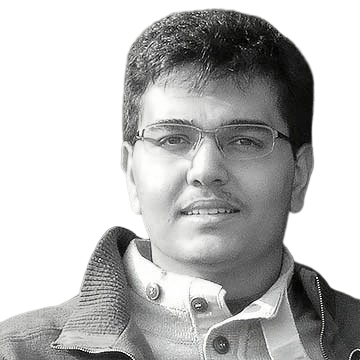
\includegraphics[width=80px]{images/farbod.png} \\
    \end{minipage}
    % Name
    % \nameTitleBox{
    \begin{minipage}[t]{3.5cm}
        \vspace{8mm}
        \noindent
        \huge\bfseries
        Farbod\\
        Shahinfar
        % \vspace{0.0cm}
    \end{minipage}
    % }
    \hfill\null
    \begin{minipage}[t]{6cm}
        \vspace{6mm}
        % Contact Information
{ % \small
% \noindent
% \flushright
\noindent
\begin{tabular}{p{8cm}l}
    Email: \href{mailto:farbod.shahinfar@polimi.it}{farbod.shahinfar@polimi.it} & 
    Web page: \href{https://fshahinfar1.github.io}{fshahinfar1.github.io} \\
    Address: Via Ponzio 34/5, 20133 Milano &  \\
    \multicolumn{2}{l}{Affiliation: Politecnico di Milano, Dipartimento di Elettronica, Informazione e Bioingengeria} \\
    % Github: \href{https://github.com/fshahinfar1}{github.com/fshahinfar1} & Birthday: 25/Feb/1998 \\
    \multicolumn{2}{l}{Research interests: Datacenter end-host systems, Network stack implementation and design}
\end{tabular}
}
% ===================================================================

    \end{minipage}
}
\vspace{-1cm}



\section{}
Studying Master of Sc. in computer engineering at Sharif university of technology.

\vspace{0.5cm}
\noindent\textbf{Research Interests:} \\
\indent  Performance of Programable Networks and Computer Systems


\section{Education}

\eduWithDetail{MSc. Computer Software Engineering}{Sharif University of Technology}{Graduating September 2022}{images/sharif.png}{
    \multilineCell {
        \hspace{5mm} \textbf{Project}:
        Optimizing Load Balancing for Serverless Computing Platforms \\
        \hspace{10mm} using Modeling Approaches \\
        \hspace{5mm} \textbf{Supervisor}: Dr. Ali Movaghar
    }
}
\vspace{-5mm}

\eduWithDetail{BSc. Computer Engineering}{Iran University of Science and Technology}{Graduated September 2020}{images/iust.png}{
    \multilineCell{
        \hspace{5mm} \textbf{Frist Rank}, 18.62/20 GPA \\
        \hspace{5mm} \textbf{Project}:
        Study of MMU Cache Partitioning Efficacy for Hierarchical Page Tables \\
        \hspace{10mm} in OS Memory Management \\
        \hspace{5mm} \textbf{Supervisor}: Dr. Mohsen Sharifi
    }
}
\vspace{-5mm}

% \eduSmall{High School Diploma}{Salam 3}{Graduated May 2015}{images/salam.png}


\section {Publication}

\begin{itemize}
    \item A. Sanaee, F. Shahinfar, B. E. Stephens, G. Antichi, ``Backdraft: a Lossless Virtual Switch that
Prevents the Slow Receiver Problem'', in NSDI 2022.

    \item F. Shahinfar, S. Miano, A. Sanaee, G. Siracusano, R. Bifulco, G. Antichi,
``The case for network functions decomposition'', in CoNext 2021.
\end{itemize}

\section{Teacher Assistant}
% IUST
\noindent \textbf{Iran University of Science and Technology} \par
September 2017 – Nov 2020
{
    \renewcommand\labelitemi{}
\begin{itemize}
    \item {\textbf{Operating Systems}  \null\hfill Fall-2020 \\ Dr. Mohsen Sharifi}
    \item {\textbf{Database design} \null\hfill Spring-2019 \\ Dr. Eisa Zarepour }
    \item {\textbf{Introduction to programming in Java} \null\hfill Spring-2019 \\
        Dr. Mohammad Taher Pilevar}
    \item {\textbf{Introduction to programming in python} \null\hfill Fall-2017 and Spring-2018 \\
 Dr. Adel Rahmani }
\end{itemize}
}

% Khatam
{
\renewcommand\labelitemi{}
\noindent \textbf{Khatam University} \par
July 2019 - September 2019
\begin{itemize}
    \item {\textbf{Python Programming Crash Course}  \null\hfill Summer-2019 \\
        Dr. Mohammad Taher Pilevar}
\end{itemize}
}


\section{Frameworks/Softwares}
\subsection{NFV \& End Host Networking}
\begin{itemize}
    \item DPDK application programming
    \item XDP \& AF\_XDP
    \item BESS: Berkeley Extensible Software Switch
    \item TAS: TCP Accelartion Service
\end{itemize}


% \subsection{Linux Programming:}
% \begin{itemize}
%     \item Linux Kernel Memory Subsystem
%     \item Developing Kernel Modules
% \end{itemize}

\subsection{Programming Languages:}
\begin{itemize}
    \setlength\itemsep{0em}
    \begin{multicols}{2}
        \item {Python}
        \item {C/C++}
        \item {Javascript}
        \item {Bash Script}
        % \item {C\#}
        % \item {Java}
        % \item {SQL}
    \end{multicols}
\end{itemize}

% \subsection{Frameworks:}
%     \emph{React Native},
%     \emph{Flask},
%     \emph{Numpy and Matplotlib}

% \subsection{Softwares:}
% \begin{itemize}
%     \setlength\itemsep{0em}
%     \begin{multicols}{2}
%     \item{Docker}
%     \item{Git}
%     \item{PostgreSQL}
%     \item{MongoDB}
%     \item{Redis \& Memcached}
%     \item{Unity3d}
%     \item{Vim}
%     \item \LaTeX
%     \end{multicols}
% \end{itemize}

% \section {Work Experience}
% % \noindent \textbf{Smart Online Monitoring Co} \par
% % Application Developer \par
% % January 2020 – Peresent \par
% % \begin{itemize}
% %     \item Developer of Kidak android application
% %     \item Develop android application with React Native framework
% %     \item Experience developing a BLE (bluetooth low energy) application
% % \end{itemize}
% % \topic{React Native}
% % \topic{Javascript}
% % \topic{BLE}
% % \vspace{15pt}
%
% \noindent \textbf{Cognia} (DigikalaNEXT Summer Camp) \par
% Backend Developer \par
% July 2019 – March 2020 \par
% \begin{itemize}
%     \item Develop data gathering and data processing service
%     \item Deploy service with containerization
% \end{itemize}
% \topic{Python}
% \topic{Flask}
% \topic{PostgreSQL}
% \topic{MongoDB}
% \topic{Redis}
% \topic{Docker \& Docker Compose}
% \topic{Locust}
% \vspace{15pt}
%
% \pagebreak
%
% \noindent \textbf{Loop Game Studio} \par
% Backend Developer (A project contract) \par
% June 2019 – August 2019 \par
% \begin{itemize}
%     \item Develop a REST API server for the game.
%     \item Design a relational database for cutsomizable items in sale.
% \end{itemize}
% \topic{Python - Flask}
% \topic{PostgreSQL}
% \topic{Docker \& Docker Compose}
% \vspace{15pt}
%
% \noindent \textbf{ElmoGame} \par
% Game developer \par
% July 2017 – January 2019 \par
% \begin{itemize}
%     \item Part of the technical team for \emph{Footyard} online game
%     \item Work with Unity3d engine
%     \item Apply software design patterns in the project
%     \item Communicate with game server using REST APIs
% \end{itemize}
% \topic{Unity3D}
% \topic{C\#}
% \vspace{15pt}

% \section{Projects}
% \begin{multicols}{2}
% \begin{itemize}
%         \item { \emph{Footyard:} An online multi-player game developed for
%                 android devices.}
% \end{itemize}
% \end{multicols}

\subsection{Languages:}
    \emph{Persian}: Native \\
    \emph{English}: Working Profeciency

\end{document}
